\section{Document Stores}

A document store, unlike a data lake, manages the data directly and the users do not see the physical layout.
\textcolor{red}{You will not have to write MongoDB code in the Exam!}

\subsection{Relational Databases}
In relational databases, everything is a table. We saw that a table can be seen as a set of maps (from attributes to values) that fulfils three constraints: relational integrity, domain integrity, and atomic integrity. It can optimize the layout of the data on disk and build additional structures (indices) to accelerate SQL queries without the need
to modify them, and it can handle transactions.

\subsection{Challenges}

\subsubsection{Schema on read}
Data that fulfills relational integrity, domain integrity, and atomic integrity always comes with a schema. In a relational database management system, it is not possible to populate a table without having defined its schema first.

When encountering such denormalized data, in the real world, there is often no schema. In fact, one of the important features of a system that deals with denormalized data is the ability to discover a schema, i.e., offer query functionality to find out which keys appear in the data, what kind of value is associated with each key, etc; or even functionality that directly infers a schema, as we saw is the case with Apache Spark.

In Document stores, you can just pour your trees into your collection, without a schema, and it will just work, even if the trees are heterogeneous. But if you want a schema, you can have one. You can either define a schema from the very beginning, and then allow the documents that fit the schema and throw an error if they don't, or you can first pour your trees into your collection, then maxbe clean it up and then validate against the schema and then force the validation forever. Thus we are not obligated to check for a schema from the beginning, we can do it later.

\subsubsection{Making trees fit in tables}

A first thought when trying to build a system that supports denormalized data, such as collections of JSON or XML objects, is to force-fit it into tables. In fact, it is a very natural thing to do if the collection is flat and homogeneous, i.e., respects the three fundamental integrity constraints.

\vspace{1\baselineskip}

\begin{minipage}{0.26\textwidth}
\begin{lstlisting}[style=json,caption={JSON Object}]
{
    "foo":      1,
    "bar":      "foo",
    "foobar":   true,
    "a":        "bar",
    "b":        3.14
}
\end{lstlisting}
\end{minipage}
\hfill
\begin{minipage}{0.3\textwidth}
\begin{lstlisting}[style=xml,caption={XML Object}]
<row>
    <foo>1</foo>
    <bar>foo<\bar>
    <foobar>true</foobar>
    <a>foo</a>
    <b>3.14</b>
</row>
\end{lstlisting}
\end{minipage}
\hfill
\begin{minipage}{0.3\textwidth}
\begin{tabular}{c|c|c|c|c}
    foo & bar & foobar & a & b \\ \hline
    1 & foo & true & foo & 3.14
\end{tabular}
\end{minipage}

The corresponding XML Schemas can also be transformed naturally to a relational schema. The same goes for JSound or JSON Schemas.

\begin{lstlisting}[style=xml,caption={XML Schema}]
<xs:schama xmlns:xs="http://www.w3.org/2001/XMLSchema">
    <xs:element name="row">
        <xs:complexType>
            <xs:sequence>
                <xs:element name="foo" type="xs:integer"/>
                <xs:element name="bar" type="xs:string"/>
                <xs:element name="foobar" type="xs:boolean"/>
                <xs:element name="a" type="xs:string"/>
                <xs:element name="b" type="xs:decimal"/>
            </xs:sequence>
        </xs:complexType>
    </xs:element>
</xs:schema
\end{lstlisting}   

\begin{lstlisting}[style=json,caption={JSON Schema}]
{
  "foo"   :   "integer",
  "bar"   :   "string",
  "foobar":   "boolean",
  "a"     :   "string",
  "b"     :   "decimal"
}
\end{lstlisting}    

This however, is generally not a great approach because semi-structured data can be nested and heterogeneous. One possible way to deal with this issue may be:

\begin{figure}[h]
    \centering
    \begin{subfigure}{0.49\textwidth}
        \centering
        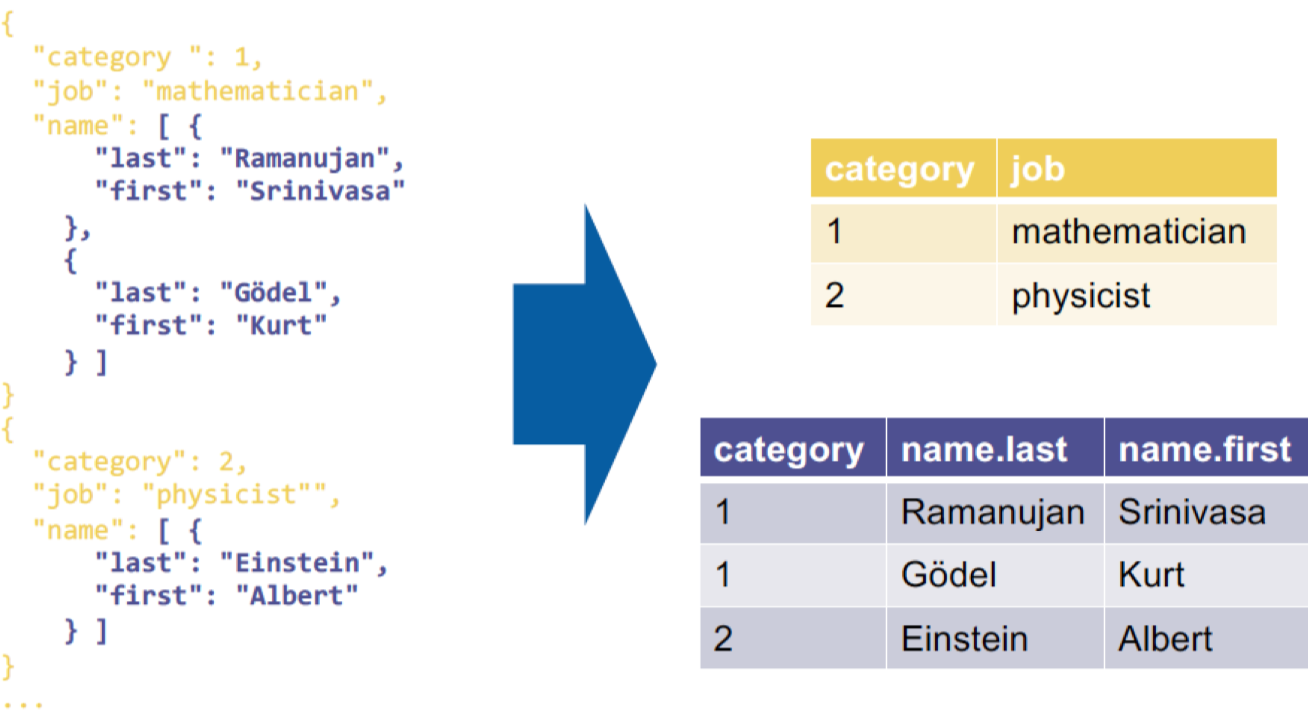
\includegraphics[width=\textwidth]{Figures/NestednessIssue.png}
        \caption{Nestedness Issue is resolved by creating two separate tables.}
    \end{subfigure}
    \hfill
    \begin{subfigure}{0.49\textwidth}
        \centering
        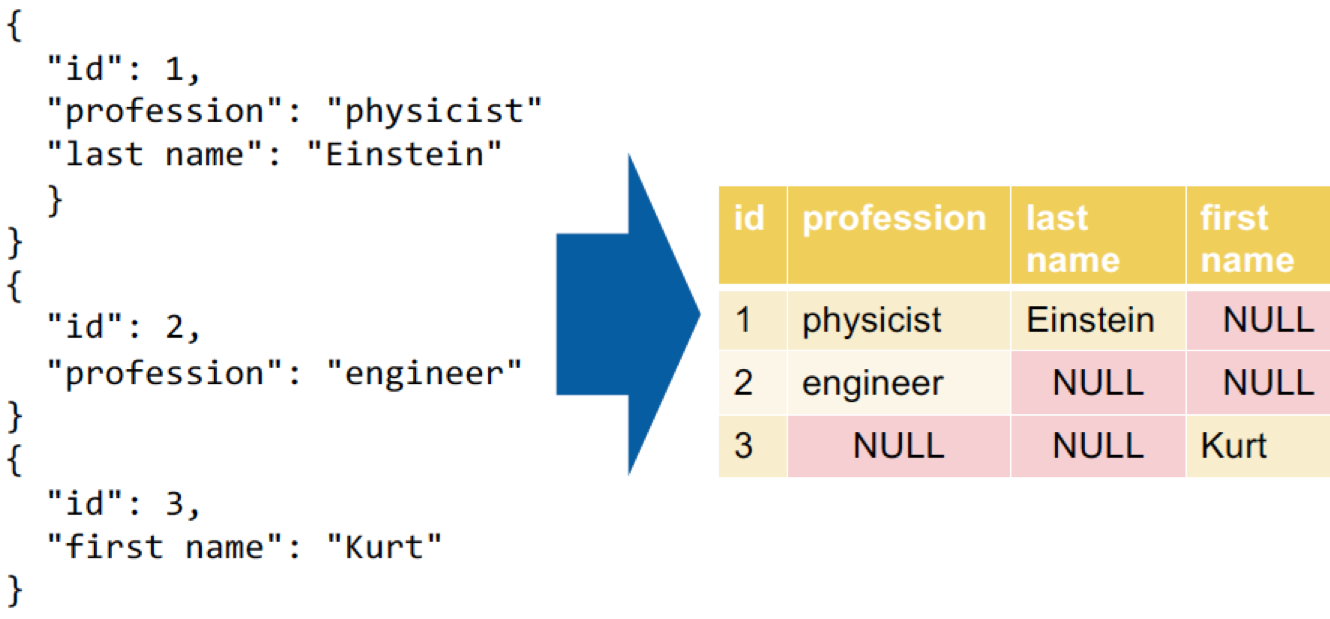
\includegraphics[width=\textwidth]{Figures/HeterogenetyIssue.png}
        \caption{Heterogeneity Issue is resolved by filling the missing values with NULL.}
    \end{subfigure}
    \caption{Nestedness and Heterogeneity Issues.}
\end{figure}

In general cases, we have a impedance mismatch. Meaning: when you have data that has a certain shape and a certain model and you try to hit it with a hammer to fit it into a different system that was designed for another shape and another model.

\subsection{Document Stores}
Document stores provide a native database management system for semi-structured data. Document stores work on collections of records, generalizing the way that relational tables can be seen as collections of rows.

Records in a document store are called documents. It is important to understand that document stores are optimized for the typical use cases of many records of small to medium sizes. Typically, a collection can have millions or billions of documents, while each single document weighs no more than 16 MB. Some document stores strictly enforce a maximum size and will not allow larger individual documents.

Finally, a collection of documents need not have a schema: it is possible to insert random documents that have dissimilar structures with no problem at all. Most document stores, however, do provide the ability to add a schema. If they do, it is then possible to validate the documents in a collection. This can be done before adding documents (schema-on-write), to ensure validity, or validation can be attempted after adding the schema to a previously schemaless collection, or while processing a collection (schema-on-read).

Document stores can generally do selection, projection, aggregation and sorting quite well, but many of them are typically not (yet) optimized for joining collections. In fact, often, their language or API does not offer any joining functionality at all, which pushes the burden to reimplement joins in a host language to the users. The same applies for complex queries that push the API to its limits and force users to write a significant part of their code in the host language, rather than push it down to the document store. This is a serious breach of data independence.


\subsubsection{Implementations}
There are many different document stores such as MongoDB, CouchDB, ElasticSearch, and many more. We will focus on MongoDB.

\subsubsection{Physical Storage}

In a data lake, the files are stored "as is" in the cloud or on a distributed file system. In a databsae management system, the storage format si typically proprietary and optimized for performance. It is hidden from the user. Just like the storage format si optimized for tabular data in a relational database management system, it is optimized for tree-like data in a cocument store.

In MongoDB, the format is a binary version fo JSON called BSON (Binary JSON). BSON is basically based on a sequence of tokens that efficiently encode the JSON constructs found in a document, like so:
\begin{align*}
    \mathrm{ \geschwungeneklammer{"foo": null} \ \Rightarrow \ 6 \ \backslash x03 \ \backslash x66 \ \backslash x6F \ \backslash x6F \ \backslash x00 \ \backslash x04 \ \backslash x00 }
\end{align*}
The immediate benefit of BSON is tha tit takes less space in storage than JSON stored as a text file. Furthermore, BSON supports additional types that JSON does not have, such as dates.

Atomicity is guaranteed on the level of documents. One can change two documents at the same time, however two users cannot access the same document at the same time.


\subsection{Querying paradigm (CRUD)}

The API of MondoDB, like many other document stores, is based on the CRUD paradigm. CRUD means Create, Read, Update, Delete and corresponds to low-level primitives.

\subsubsection{Populating a collection}
Collections in MongoDB are accessed in JavaScript via \texttt{db.scientists} where "scientists" is the name of the collection. You can insert one document with the method
\begin{lstlisting}[style=neutral]
db.scientists.insertOne(
    {
        "Last" : "Einstein",
        "Theory" : "Relativity"
    }
)
\end{lstlisting}

In order to insert several documents at the same time you can use:

\begin{lstlisting}[style=neutral]
db.scientists.insertMany(
    [
        {
            "Last" : "Lovelace",
            "Theory" : "Analytical Engine"
        },
        {
            "Last" : "Einstein",
            "Theory" : "Relativity"
        }
    ]
)
\end{lstlisting}

MongoDB automatically adds to every inserted document a special field called "\_id" and associates with a value called Object ID and with a type of its own. An Object ID can simply be thought of as a 12 byte binary value. Object Ids are convenient for deleting or updating a specific document with no ambiguity.

\subsubsection{Querying a collection}

\paragraph{Scan a collection}
Asking for the content of an entire collection is done via \texttt{db.collection.find()}. Equivalently in SQL:
\begin{lstlisting}[style=neutral]
SELECT *
FROM collection
\end{lstlisting}
This function does not in fact return the entire collection; rather, it returns some pointer, called a cursor, to the collection; the user can then iterate on the cursor in an imperative fashion in the host language (this is another reason why this is not a query language).

\paragraph{Selection}
You can perform a selection by passing one or more parameters to \texttt{find()}:
\begin{lstlisting}[style=neutral]
db.collection.find({"Theory" : "Relativity"})
db.collection.find(
    {
        "Theory" : "Relativity",
        "Last" : "Einstein"
    }
)
\end{lstlisting}
The first of the above above query returns all documents in the collection that have a key called “Theory” associated with the string value “Relativity”. The two above queries would correspond, in SQL, to a WHERE clause, like so:
\begin{lstlisting}[style=neutral]
SELECT *
FROM collection
WHERE Theory = "Relativity"

SELECT *
FROM collection
WHERE Theory = "Relativity"
  AND Last = "Einstein"
\end{lstlisting}

What is different from a relational database, then? In a document store, it is possible that some documents have this key, while others do not. The latter are excluded from the results. It is also possible that some documents have the key, but the value is something else than a string (a number, a date, etc). These documents would also be excluded from the results.

A disjunction (OR) uses a special MongoDB keyword, prefixed with a dollar sign:
\begin{lstlisting}[style=neutral]
db.collection.find(
    {
        "$or" : [
            {"Theory" : "Relativity"},
            {"Last" : "Einstein"}
        ]
    }
)
\end{lstlisting}

MongoDB offers many other keywords, for example for comparison other than equality:

\begin{lstlisting}[style=neutral]
db.collection.find(
    {
        "Publications" : { "$gte" : 100}
    }
)
\end{lstlisting}
Equivalent to:
\begin{lstlisting}[style=neutral]
SELECT *
FROM scientists
WHERE Publications >= 100
\end{lstlisting}


\paragraph{Projection}
Projections are made with the second parameter of this same find() method. This is done in form of a JSON object associating all the desired keys in the projection with the value 1.

\begin{lstlisting}[style=neutral]
db.scientists.find(
    {"Theory" : "Relativity"},
    {"First" : 1 , "Last" : 1}
)
\end{lstlisting}

Equivalently in SQL:
\begin{lstlisting}[style=neutral]
SELECT First, Last
FROM scientists
WHERE Theory = 'Relativity'
\end{lstlisting}

By default, the object ID, in the field “ id” is always included in the results. It is possible to project it away with a 0:
\begin{lstlisting}[style=neutral]
db.scientists.find(
    {"Theory" : "Relativity"},
    {"First" : 1 , "Last" : 1, "_id" : 0}
)
\end{lstlisting}
There is no SQL equivalent for this query. It is also possible to project fields away in the same way with 0s, however 1s and 0s cannot be mixed in the projection parameter, except in the specific above case of projecting away the object ID.

\paragraph{Counting} can be done via
\begin{lstlisting}[style=neutral]
db.scientists.find(
    { "Theory" : "Relativity" }
).count()
\end{lstlisting}
equivalently in SQL:
\begin{lstlisting}[style=neutral]
SELECT COUNT(*)
FROM scientists
WHERE Theory = "Relativity"
\end{lstlisting}

\paragraph{Sorting} can be done via
\begin{lstlisting}[style=neutral]
db.scientists.find(
    { "Theory" : "Relativity" },
    { "First" : 1, "Last" : 1 }
).sort({
    "First" : 1,
    "Name" : -1
})
\end{lstlisting}
equivalently in SQL:
\begin{lstlisting}[style=neutral]
SELECT First, Last
FROM scientists
WHERE Theory = "Relativity"
ORDER BY First ASC, Name DESC
\end{lstlisting}
1 stands for ascending order and -1 for descending order. You can also add for example \texttt{.skip(30).limit(10)} after the \texttt{.sort(...)} statement which is eqiuvalent to adding the following in SQL
\begin{lstlisting}[style=neutral]
LIMIT 10
OFFSET 30    
\end{lstlisting}

\paragraph{Duplicate Elimination}
You can obtain distinct values for one field with \texttt{db.scientists.distinct("Last")}.


\subsubsection{Querying for heterogeneity}

\paragraph{Absent fields}

You can also filter for the null object. It returns all objects with either the null object as the element or the objects with no entry for that argument.
\begin{lstlisting}[style=neutral]
db.scientists.find(
    {"Theory" : null}
)
\end{lstlisting}

Equivalently in SQL:
\begin{lstlisting}[style=neutral]
SELECT *
FROM scientists
WHERE Theory IS NULL
\end{lstlisting}

\paragraph{Filtering for values across types}
Querying for several values with different types and in the same field can easily be made with a disjunctive query:
\begin{lstlisting}[style=neutral]
db.collection.find(
    {
        "$or" : [
            { "Theory" : "Relativity" },
            { "Theory" : 42 },
            { "Theory" : null }
        ]
    }
) 
\end{lstlisting}

or alternatively
\begin{lstlisting}[style=neutral]
db.scientists.find(
    {
        "Theory" : {
            "$in" : [ "Relativity", 42, null ]
        }
    }
)
\end{lstlisting}


\subsubsection{Querying for Nestedness}

\paragraph{Values in nested objects}
MongoDB uses the dot syntax. This means that, like the dollar sign, dots are treated in a special way in MongoDB queries.
\begin{lstlisting}[style=neutral]
db.scientists.find({
    "Name.First" : "Albert"
})
\end{lstlisting}
The following is \underline{false}:
\begin{lstlisting}[style=neutral]
db.scientists.find({
    "Name" : {"First" : "Albert"}
})
\end{lstlisting}
This would only return the documents in which "Name" exactly matches \texttt{\{"First" : "Albert"\}}. The above query returns all the elements that \underline{contain} "Albert" as first name.

\paragraph{Values in nested arrays}
MongoDB allows to filter documents based on whether a nested array contains a specific value, like so:
\begin{lstlisting}[style=neutral]
db.scientists.find({
    "Theories" : "Special relativity"
})
\end{lstlisting}


\subsubsection{Deleting Objects from a Collection}
You can delete one or many objects from a collection by
\begin{lstlisting}[style=neutral]
db.scientists.deleteMany(
    {"century" : "15"}
)
\end{lstlisting}
or
\begin{lstlisting}[style=neutral]
db.scientists.deleteOne(
    {"century" : "15"}
)
\end{lstlisting}
The \texttt{deletaMany} command will delete \textit{all} documents matching the criteria. The \texttt{deletaOne} command will delete just one document matching the criterion, leaving any other documents matching the criterion unchanged in the original collection. If there is no such document, nothing happens.

\subsubsection{Updating Objects in a Collection}
Documents can be updated with \texttt{updateOne()} and \texttt{updateMany()} by providing both a filtering criterion (with the same syntax as the first parameter of find()) and an update to apply.
\begin{lstlisting}[style=neutral]
db.scientists.updateMany(
    {"Last" : "Einstein"},
    {$set : {"Century" : "20"}}
)
\end{lstlisting}
In addition to \$set, there are also \$unset to remove a value and \$replaceWith to completely change an entire document.
The granularity of updates is per document, that is, a single document can be updated by at most one query at the same time. However, within the same collection, several different documents can be modified concurrently by different queries in parallel.


\subsubsection{Complex Pipelines}

For grouping and such more complex queries, MongoDB provides an API in the form of aggregation pipelines:
\begin{lstlisting}[style=neutral]
db.scientists.aggregate(
    {$match : {"Century" : 20}},
    {$group : {
        "Year" : "$year$,
        "Count" : { "$sum" : 1}
        }
    }
    {$sort : {"Count" : -1}},
    {$limit : 5}
)
\end{lstlisting}
This is somewhat a "mini Spark Implementation" in MongoDB. In SQL one could write this as
\begin{lstlisting}[style=neutral]
SELECT Year, SUM(Count) AS Count
FROM scientists
WHERE Century = 20
GROUP BY Year
ORDER BY SUM(Count) DESC
LIMIT 5
\end{lstlisting}

\subsection{Architecture}

Principle: Scaling out the hardware to multiple machine, and sharding as well as replicating the data.

\subsubsection{Sharding Collections}
Collections in MongoDB can be sharded. Shards are determined by selecting one or several fields. (Lexicographically-ordered) intervals over these fields then determine the shards. This is similar in spirit to regions in HBase, which are sharded by Row ID intervals. Shards then are stored in different physical locations. The fields used to shard must be organized in a tree index structure.

\subsubsection{Replica Sets}
A replica set is a set of several nodes running the MongoDB server process. The nodes within the same replica set all have a copy of the same data. Note that this architecture is not the same as that of HDFS, in which the replicas are spread over the entire cluster with no notion of “walls” between replica sets and no two DataNodes having the exact same block replicas. It is also not the same as HBase, in which nodes receive the responsibility of handling specific regions, but do not necessarily store them physically as this is done on the HDFS level.

\begin{figure}[h]
    \centering
    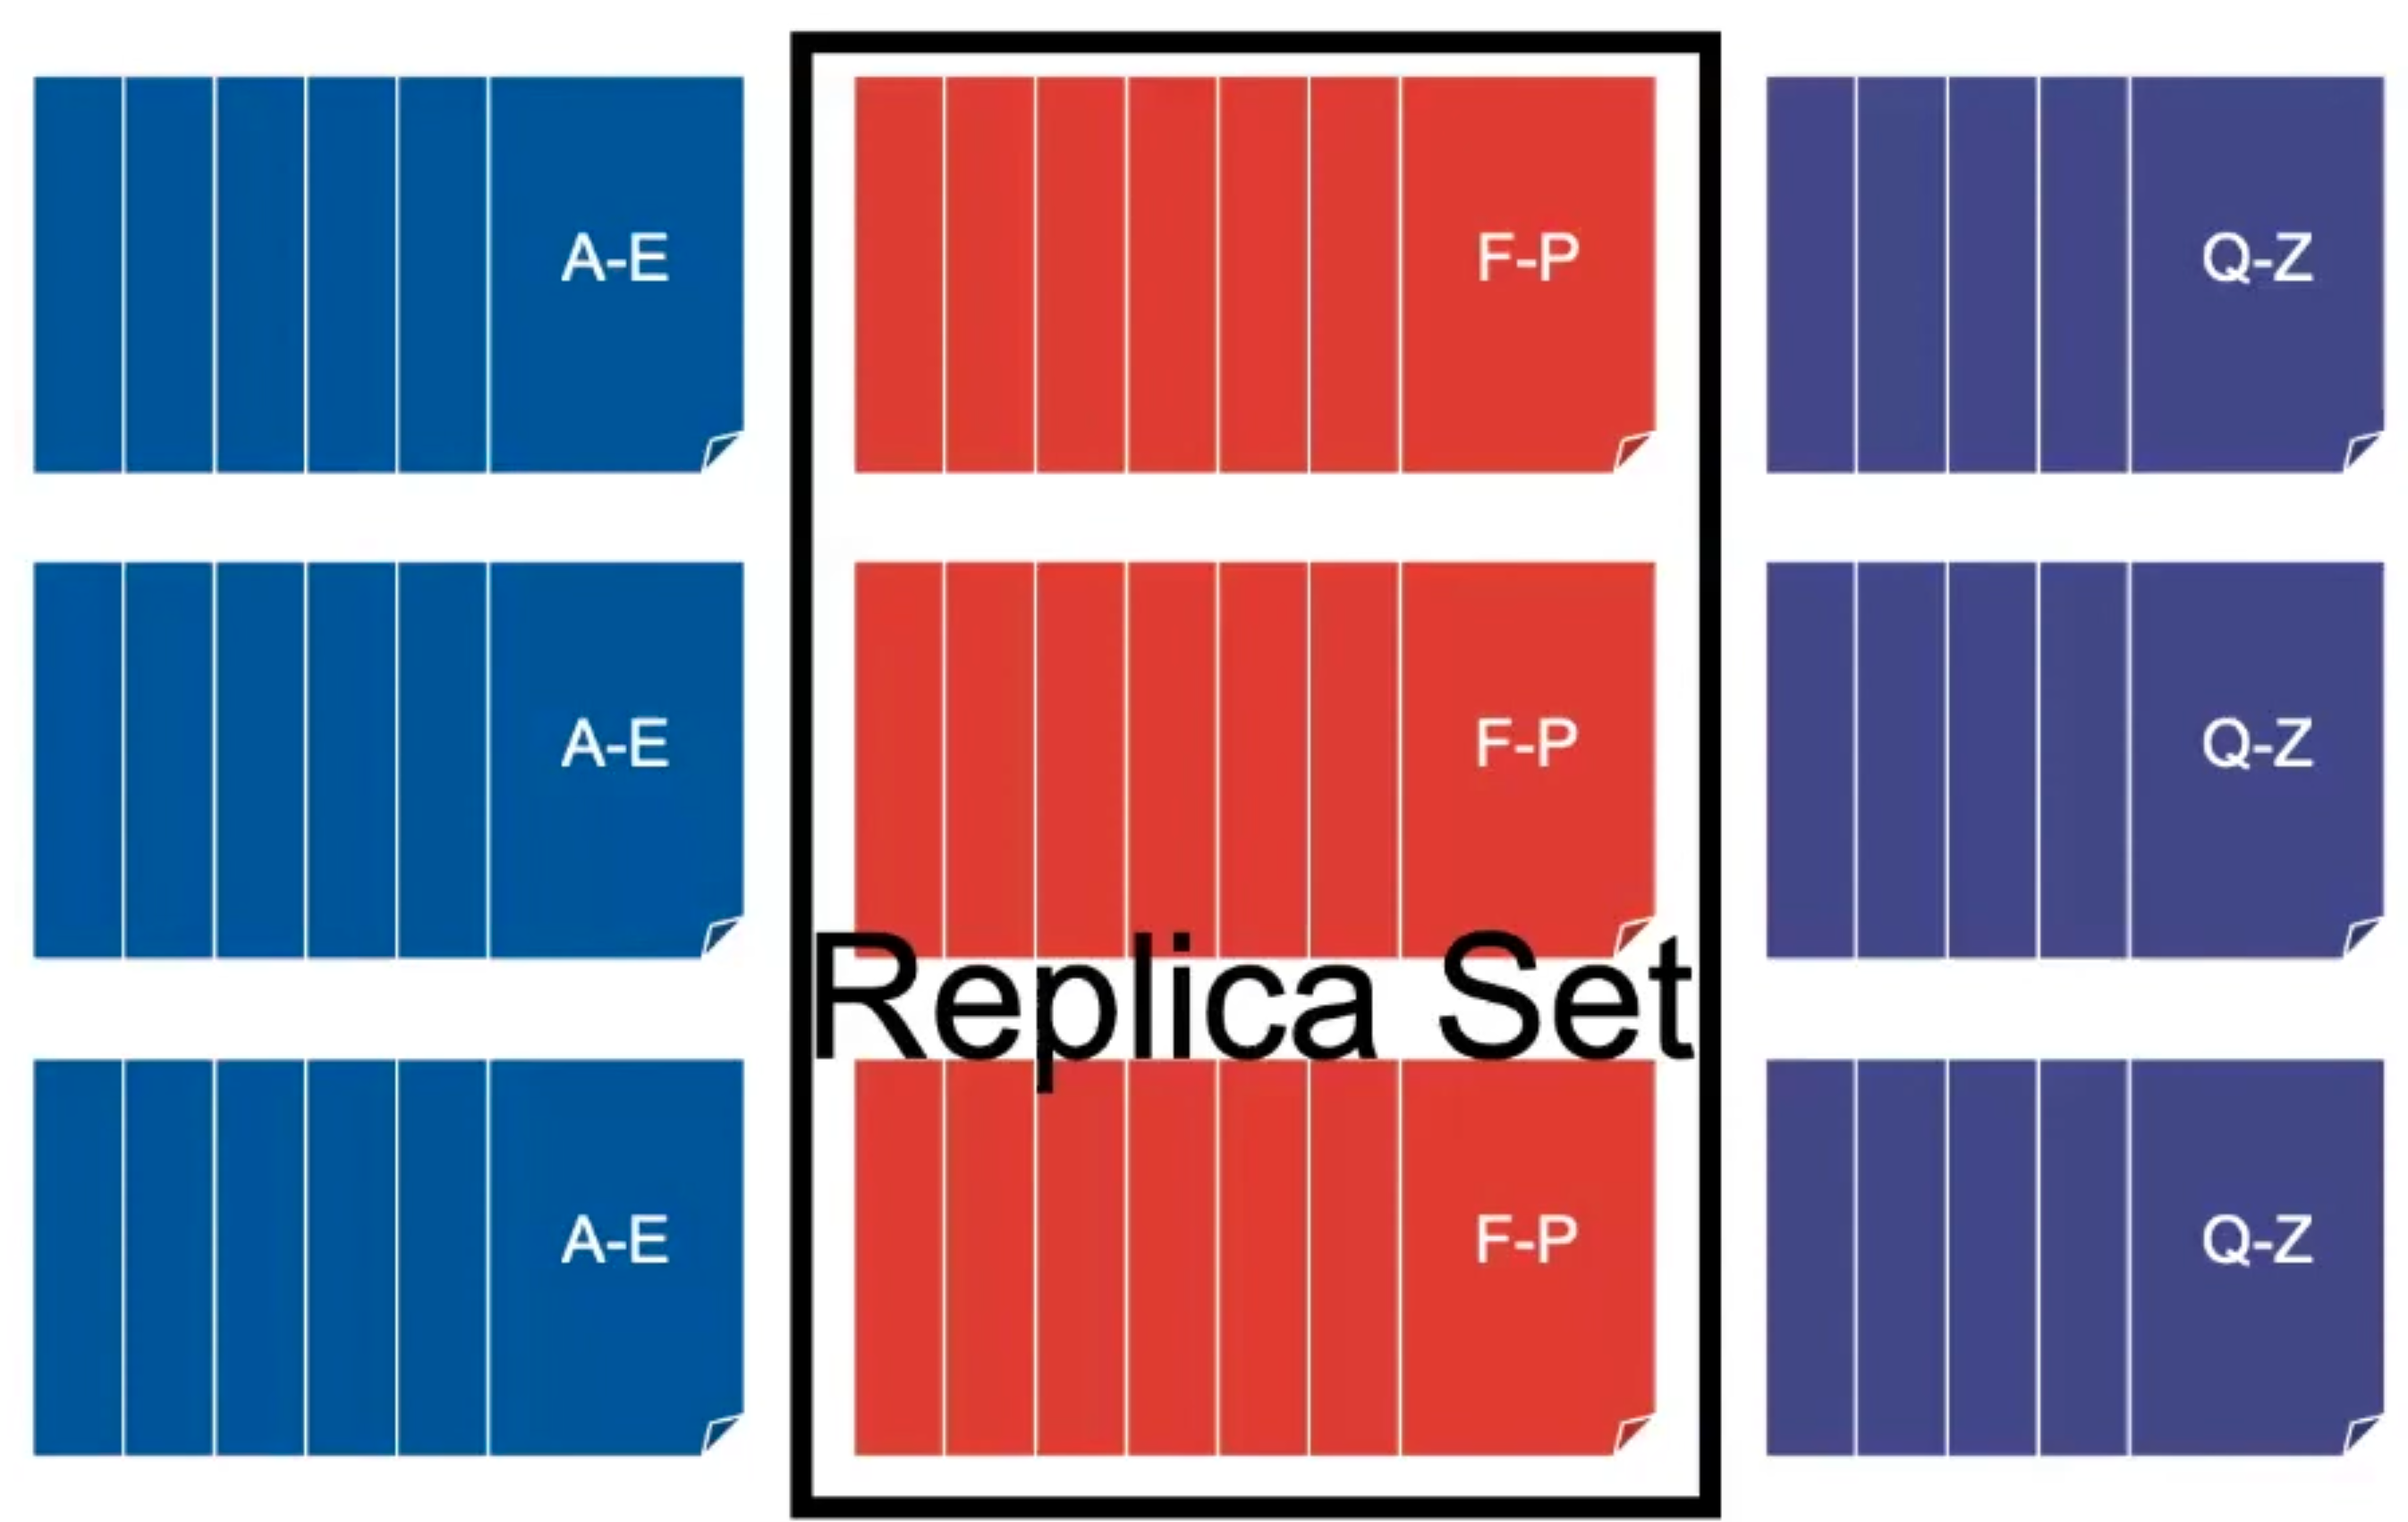
\includegraphics[width=0.5\textwidth]{Figures/DocumentStoresReplicas.png}
    \caption{Replicatoin happens vertically, and sharding horizontally.}
\end{figure}

\begin{figure}[h]
    \centering
    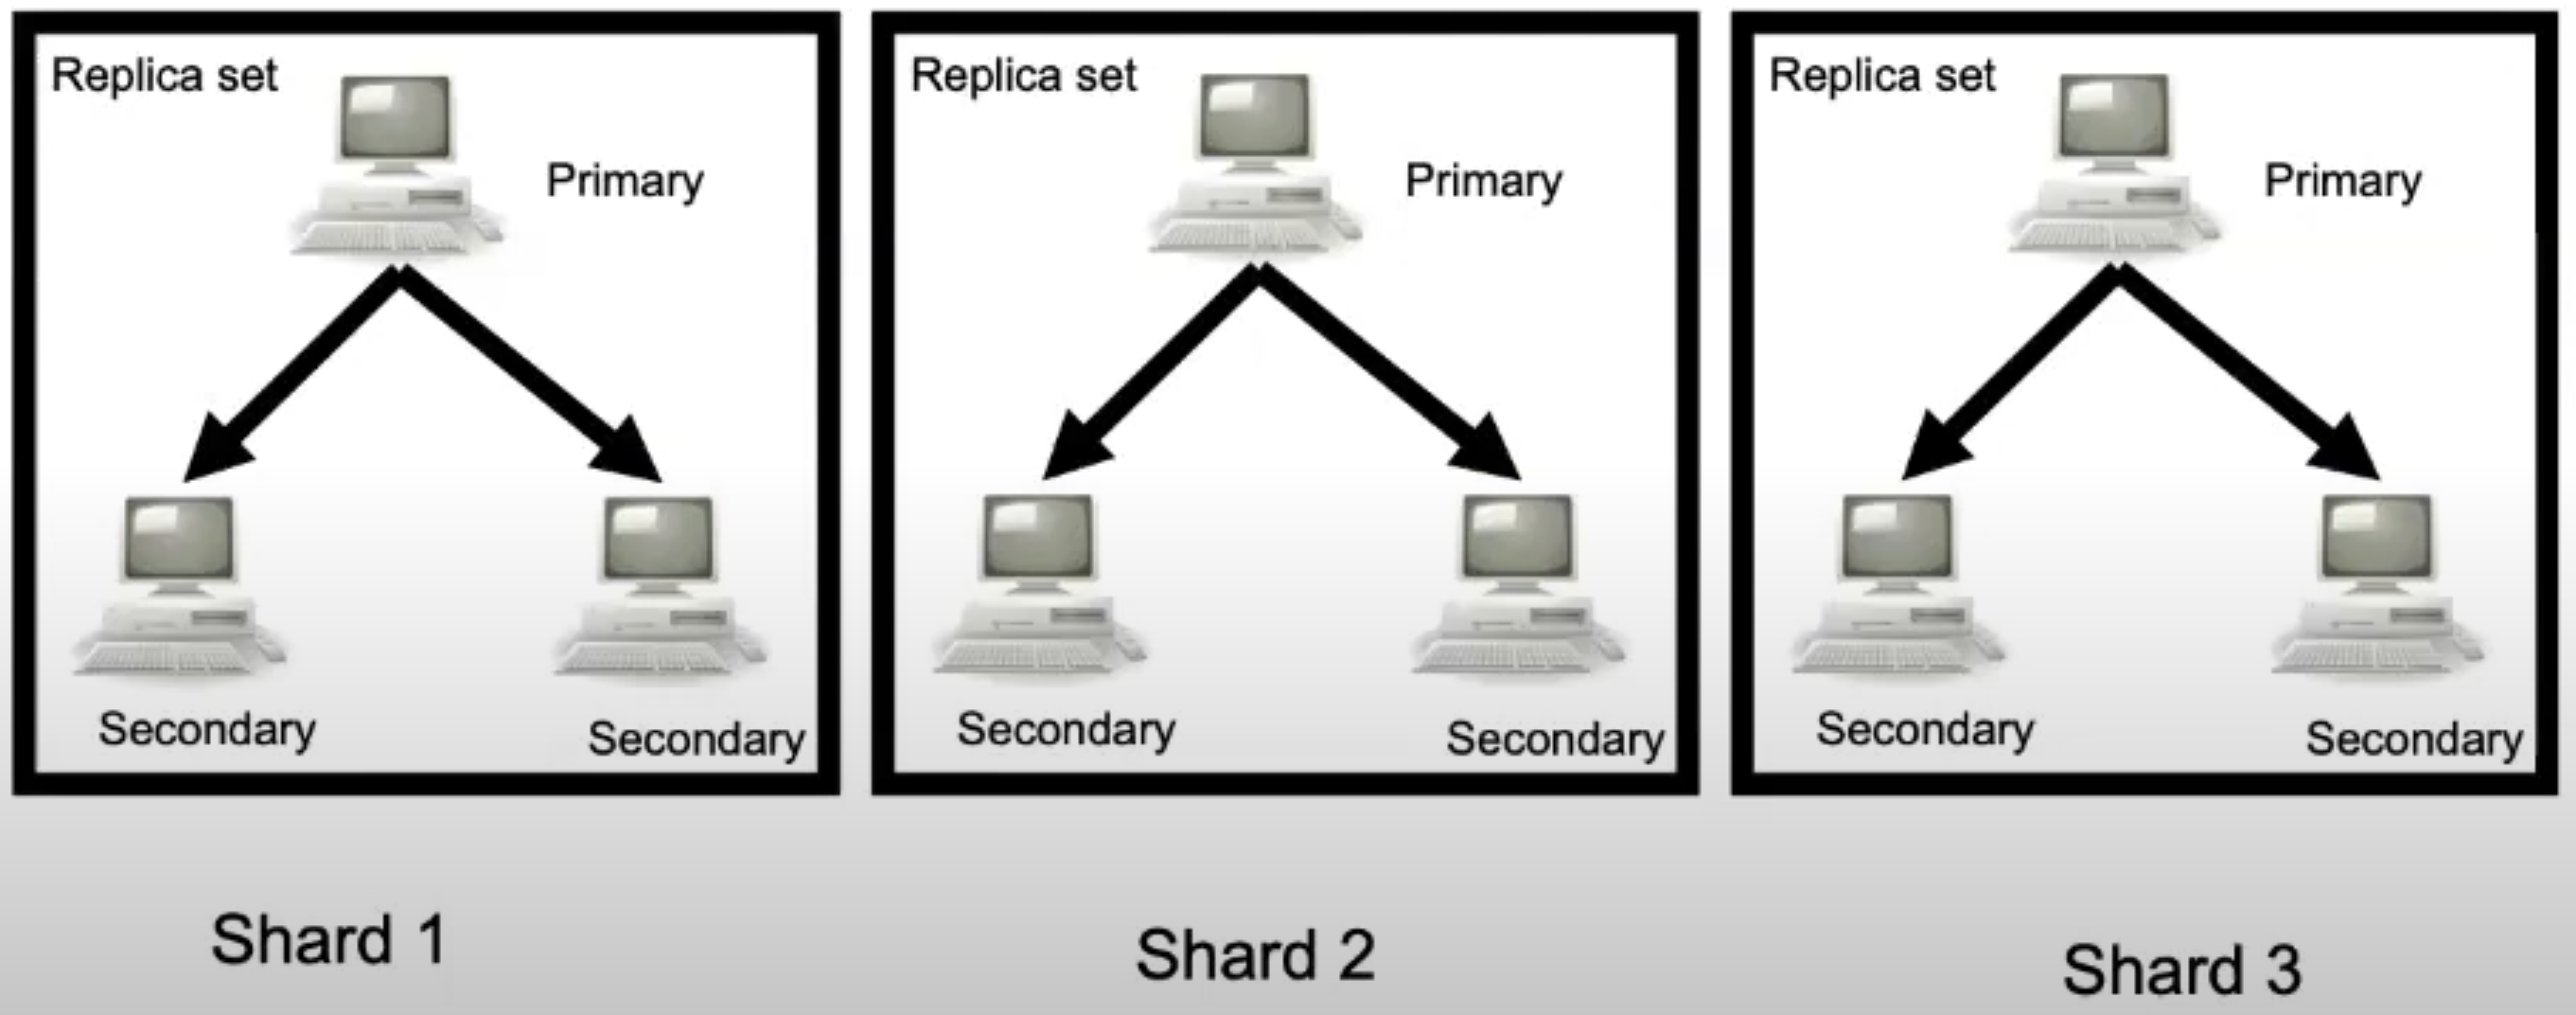
\includegraphics[width=0.8\textwidth]{Figures/DocumentStoresReplicas2.png}
    \caption{We have a coordinator node in each shard and we have worker nodes. With this we defete crashes, we don't lose data, and we can process in parallel.}
\end{figure}

\subsubsection{Write Concerns}
When writing (be it delete, update or insert) to a collection, more exactly, to a specific shard of a collection, MongoDB checks that a specific minimum number of nodes (within the replica set that is responsible for the shard) have successfully performed the update. Once the minimum number of replication is reached, the user call returns (synchronous). Then replication continues in the background to more (asynchronous).


\subsection{Indices}

\subsubsection{Motivation}
A document store, unlike a data lake, manages the physical data layout. This has a cost: the need to import (ETL) data before it is possible to query it, but this cost comes with a nice benefit: index support, just like relational database management systems.

There are different ways to look up data. Either with a point query (e.g. \texttt{find({"Name":"Euler"})}) which points to a unique document, a selection query (e.g. \texttt{find("Profession":"Mathematician")}) which points to several documents, or a range query (e.g. \texttt{find("Year":{"\$gte":1900})}).

To understand Indices, have a look at \cref{fig:Indices}. Imagine you add a structure to the list of documents, here a list of colors, sorted in a certain way, with pointers to the elements that contain that color in the document. Like this, you can lookup for example "orange" in the color list and then obtain all the pointers to the documents containing "orange" in the "Color" list. It then suffices to follow the pointer(s) to the documents with that color, which is just a disk read away.

\begin{figure}[h]
    \centering
    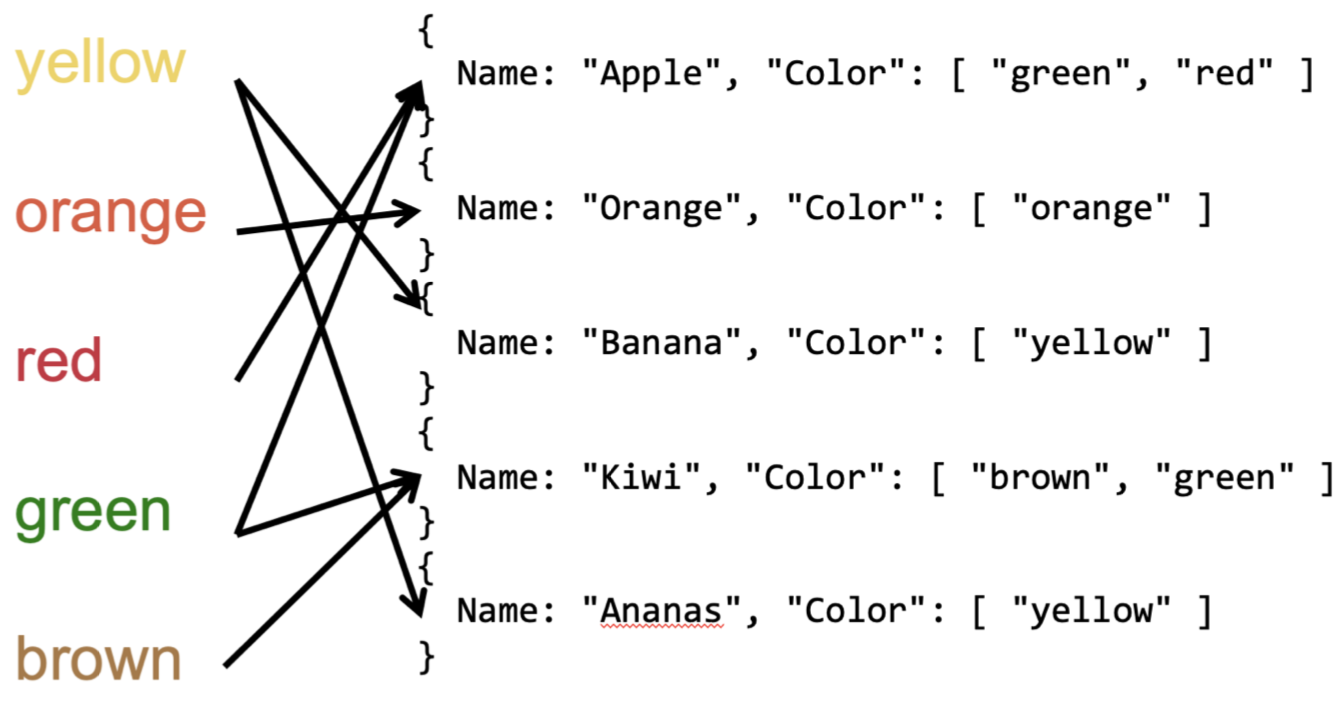
\includegraphics[width=0.7\textwidth]{Figures/Indices.png}
    \caption{Index Pointers.} \label{fig:Indices}
\end{figure}

\subsubsection{Hash Indices}

Hash indices are used to optimize point queries and more generally queries that select on a specific value of a field. The general idea is that all the values that a field takes in a specific collection can be hashed to an integer. The value, together with pointers to the corresponding documents, is then placed in a physical array in memory, at the position corresponding to this integer (modulo the
overall size of the array).

\begin{figure}[h]
    \centering
    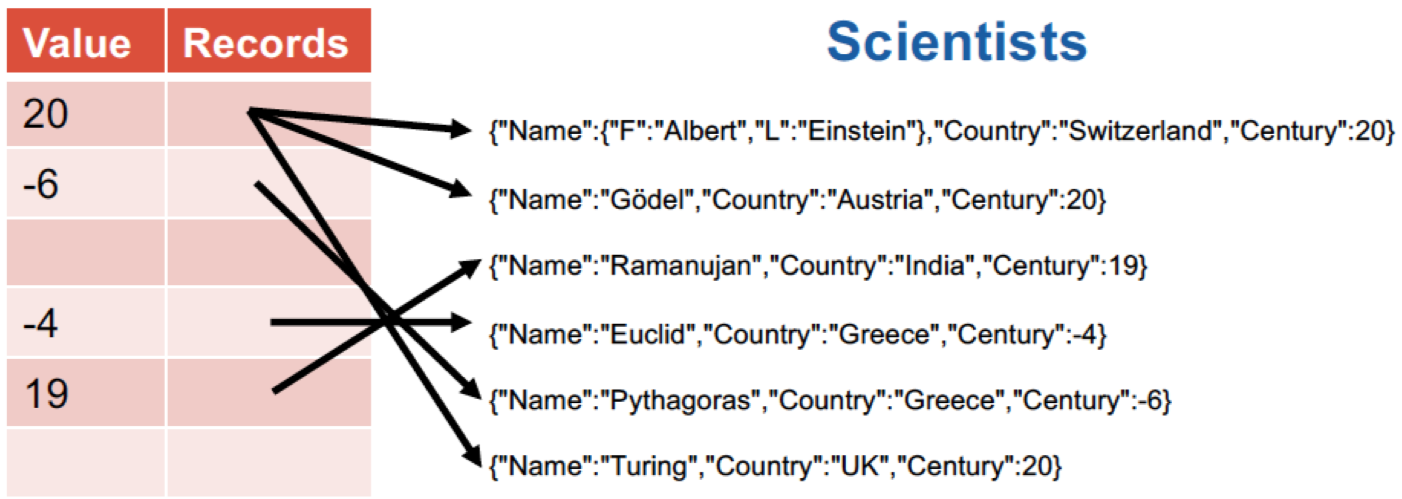
\includegraphics[width=0.6\textwidth]{Figures/HashIndexing.png}
    \caption{Hash Indices. A hash function $h$ maps the values of "Century" to an index. Here, for example $h(20)=0$, $h(-6)=1$, $h(-4) = 3$ and $h(19)=4$. Important to remember: $h$ is deterministic.}
\end{figure}

The hard part is creating the hash function $h$. Having done that, one can query extremely fast the documents in the document list. Here a code to create the hash function $h$:
\begin{lstlisting}[style=neutral]
db.scientists.createdIndex({
    "Century" : "hash"
})
\end{lstlisting}

and here a code to look up documents in the document list:
\begin{lstlisting}[style=neutral]
db.scientists.find({"Century":19})
\end{lstlisting}

Hash functions fulfill useful criteria such as making collisions unlikely, spreading values uniformly in the index array, etc. They are, in fact, more powerful than what we need, but most importantly enough powerful for what we need. Furthermore, they are very fast.

However, there is no free lunch: before an index can be used, it must be built. Building an index consists in the creation of the array structure, and then its population by sequentially scanning through the entire collection, computing the hash of the value, and adding to the index an entry and a pointer to the document, document by document.

Indices are built at the request of the user, by executing a command. Building an index can either happen synchronously, in the sense that the entire collection (or data store) remains unavailable during build time. Or it can happen asynchronously, meaning that the collection (or data store) remains available, but will be slower until the index is completely built.

\paragraph{Limitations of Hash Indices}

Hash indices to not support range queries, Hash functions are not perfect (there shouldn't be collisions, however, in real life there sometimes are collsions making it slower) and you also need a large amount of space to avoid collisions (collision means two values give the same position).

\subsubsection{Tree Indices}

Range queries are supported with tree indices. Instead of an array, tree indices use some sort of tree structure in which they arrange the possible values of the indexed field, such that the values are ordered when traversing the tree in a depth-first-search manner.

More precisely, the structure is called a B+-tree. Unlike a simple binary tree, nodes have a large number of children. The intent is that the leaves (and nodes) of the tree are large enough to match roughly a disk block, in order to optimize disk latency when fetching the nodes. In many cases, indices are so large (or numerous) that they do not fit in memory, and the database system only loads the parts of the index it needs. With nodes the size of a block, fewer disk accesses are needed.

In B+Trees it is like looking something up in a dictionary. In the example of \cref{fig:BTrees}, you look if hour is to the left or right of certain nodes. Like this, you do not need to scan the whole data. The big advantage is that you can access the data block-wise instead of bit-by-bit.

\begin{figure}[h]
    \centering
    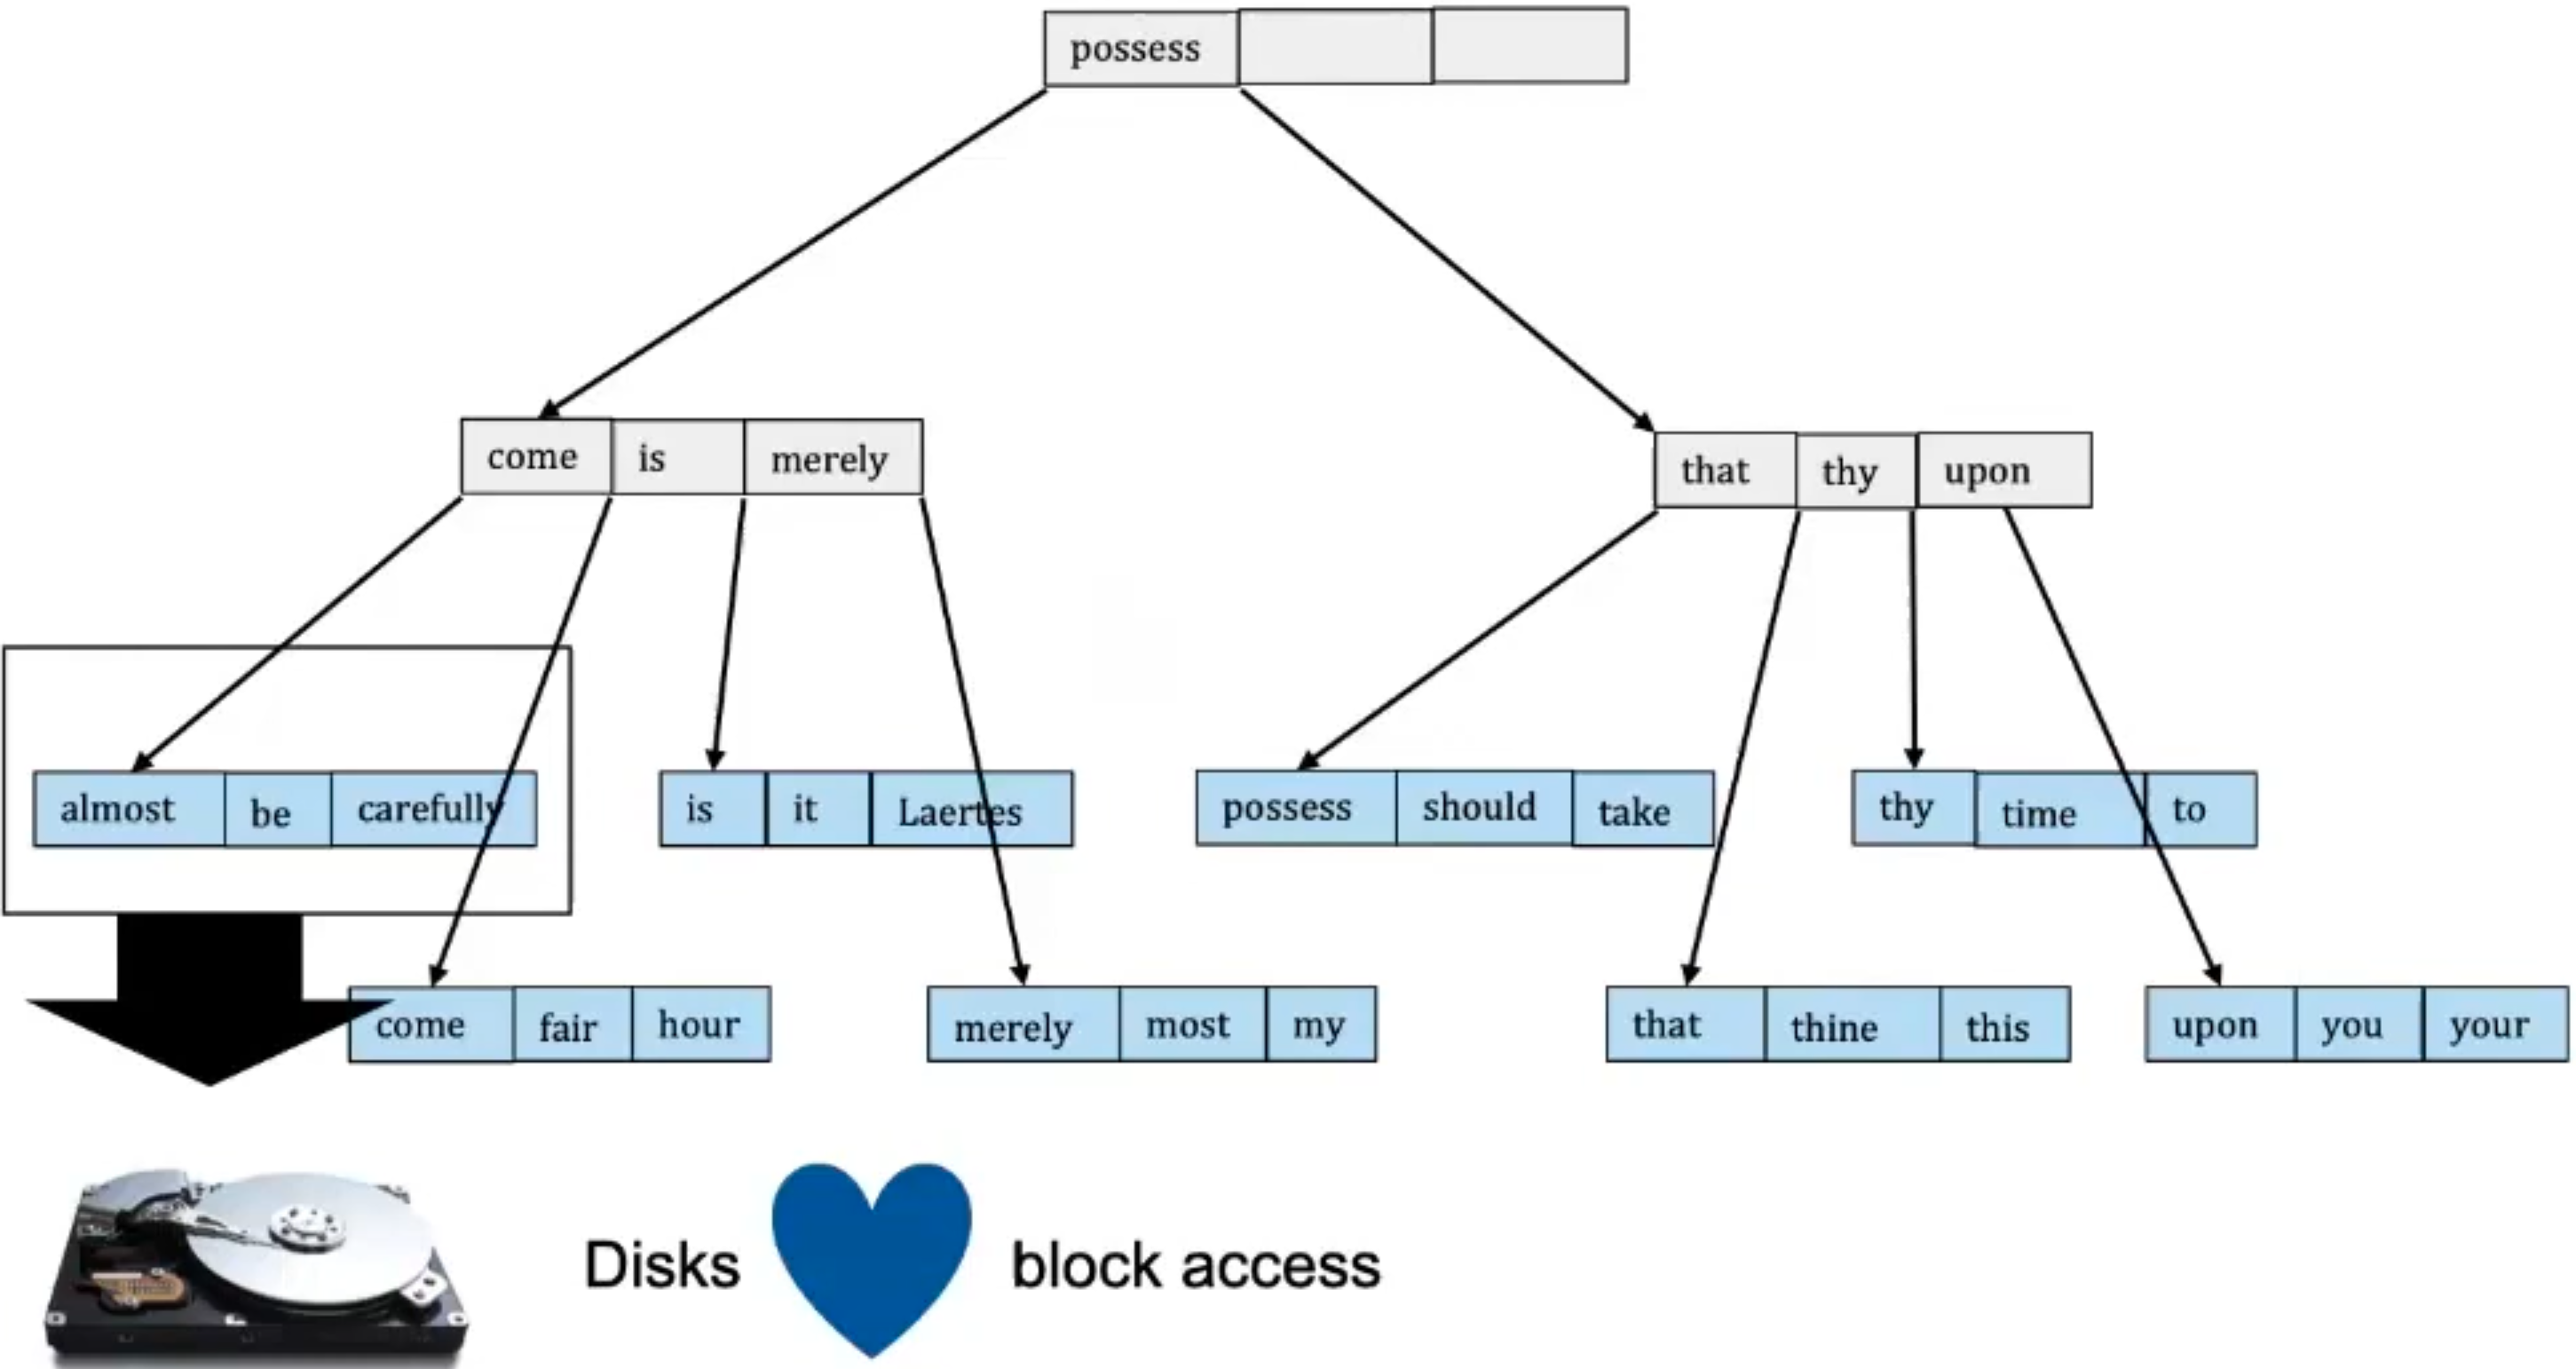
\includegraphics[width=0.7\textwidth]{Figures/B+Trees.png}
    \caption{B+Trees Illustration}\label{fig:BTrees}
\end{figure}

The code looks like this:
\begin{lstlisting}[style=neutral]
db.scientists.createIndex({
    "Century" : 1
})
\end{lstlisting}

By looking at \cref{fig:BTrees2} it is clear that range lookups are now possible. You can check for the index where for example $19$ is contained and then take all the pointers associated with the nodes to the right of the node corresponding to $19$.

\begin{figure}[h]
    \centering
    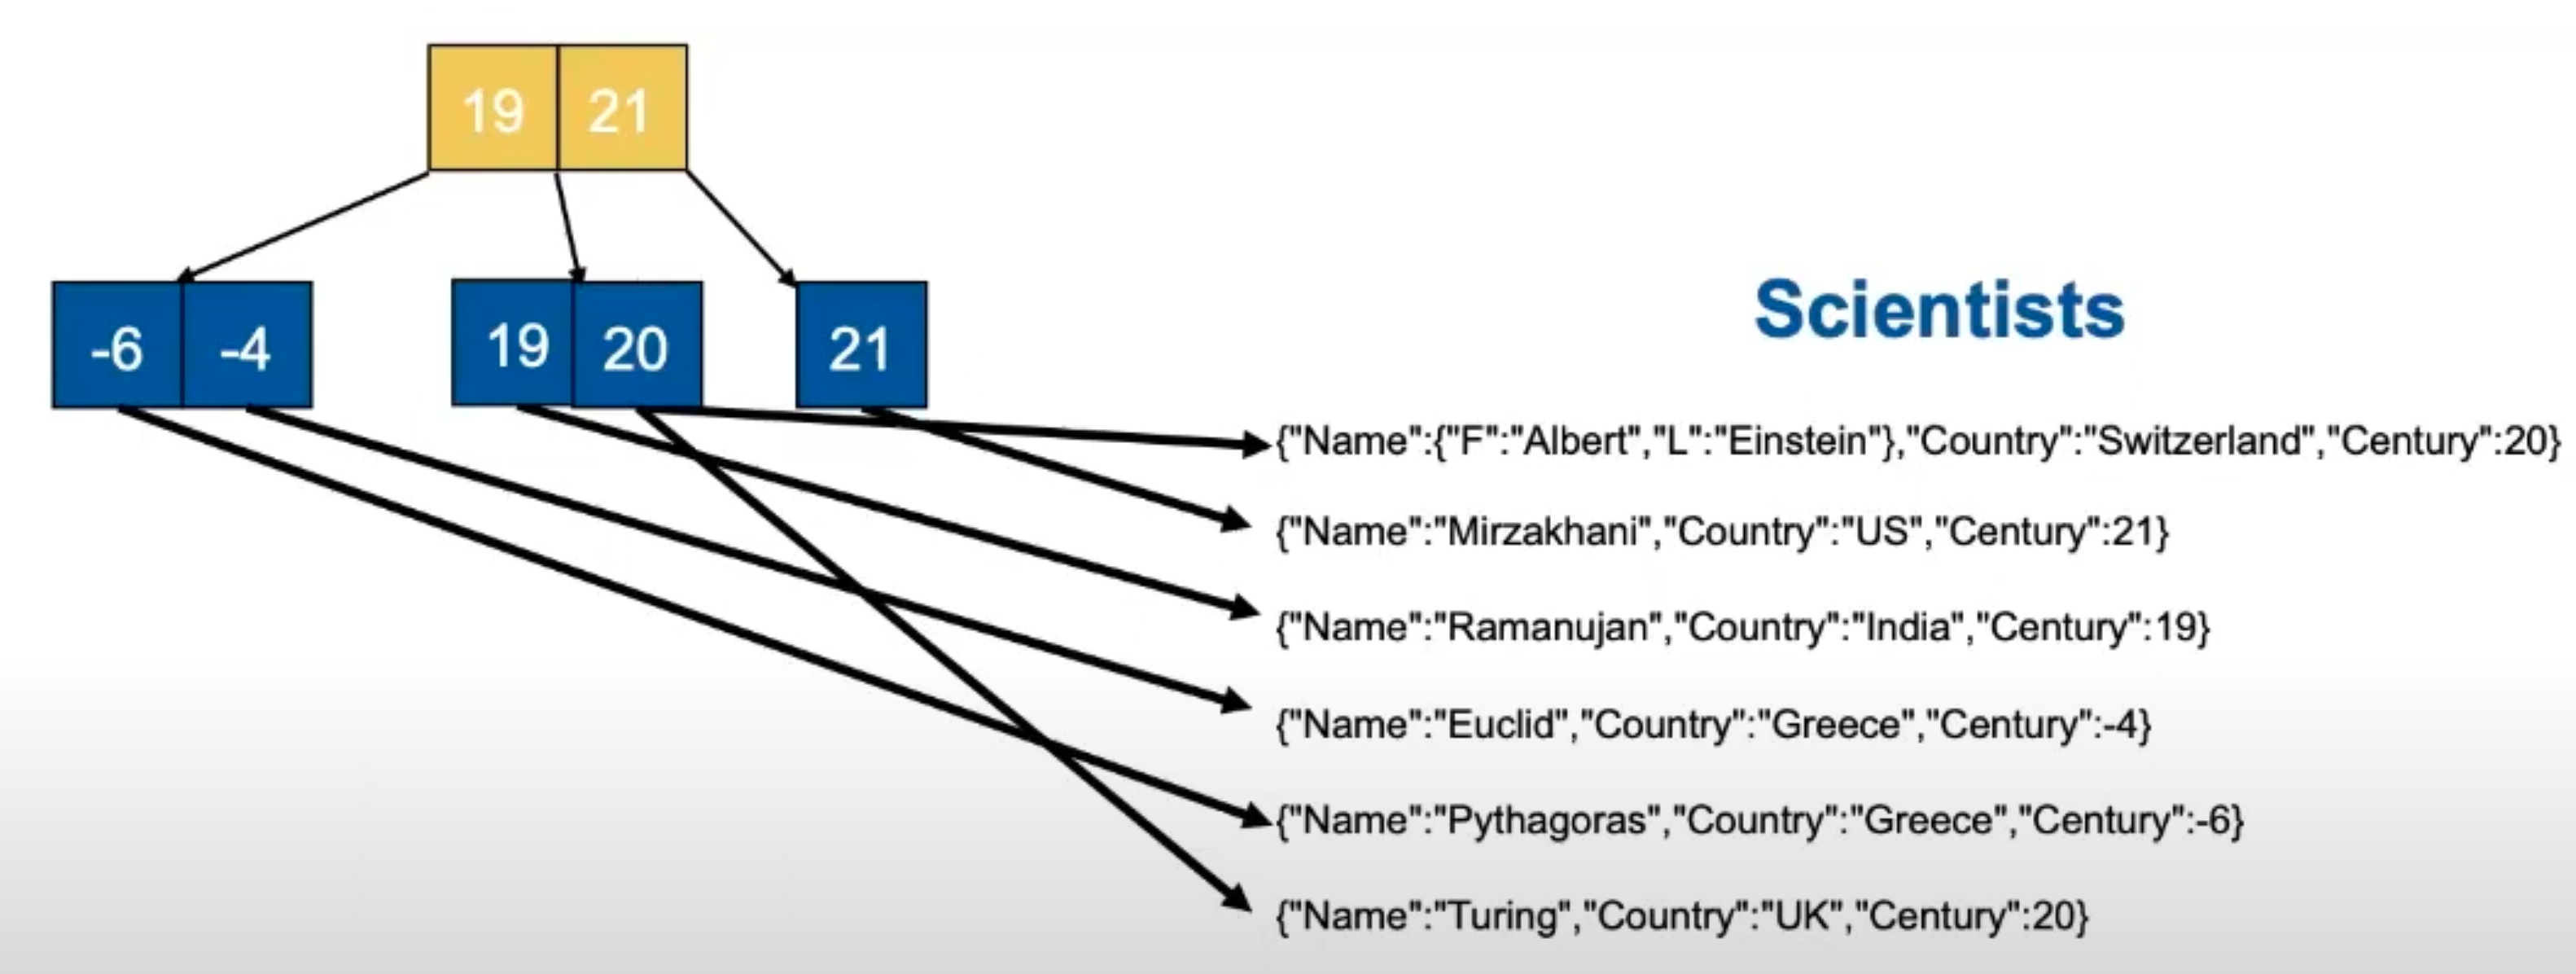
\includegraphics[width=0.7\textwidth]{Figures/BTrees.png}
    \caption{Creation of the splittings. In this example, we do not allow for blocks longer than 2. Thus, each leaf node may only have 2 elements in total. When a childnode exceeds the maximum number of elements, a new parent node is created together with another leaf containing the new datapoint. The whole tree is created in this manner. One just needs to specify how many datapoints should be in the leaf nodes. This is usually limited by memory size.}\label{fig:BTrees2}
\end{figure}

There are a few constraints in a B+-tree. First, all leaves must be at exactly the same depth. This depth grows with larger collections. Second, the number of children of each node must be within a specific interval, generally parameterized as between d + 1 and 2d + 1 with some choice of d. For pedagogical purposes, we use a small value of d on our examples, but in practice d is larger. The only exception is the root node, which is not subject to the d + 1 minimum. The root can have less children, but at least two (had it only one child, it would be useless and could be removed).

The non-leaf nodes in the tree contain a list of increasing values, interlaced with pointers to the children. These values are compared to the actually sought value in order to locate the pointer that must be followed in order to resolved this sought value. There is exactly one less value on a node than its number of children. Thus, each node has between d and 2d values.

In a B+-tree, all possible values appear on the leaves together with a pointer to the documents that contain them. The values can be “repeated” on non-leaf nodes, but values on non-leaf nodes are only used for comparison purposes. A B+-tree also typically chains all its leaves with pointers, for efficient full-traversals in ascending value order. This allows resolving a range query by only looking up the bounds in the B+-tree, and then traversing from the minimum to the maximum value.

This is unlike B-trees, in which non-leaf nodes can also contain pointers to documents.

\subsubsection{Secondary Indices}

You can create indices on secondary entries:

\begin{lstlisting}[style=neutral]
db.scientists.createIndex({
    "Name.Last" : "hash"
})
\end{lstlisting}
or
\begin{lstlisting}[style=neutral]
db.scientists.createIndex({
    "Name.Last" : 1
})
\end{lstlisting}
or when involving several fields
\begin{lstlisting}[style=neutral]
db.scientists.createIndex({
    "Name.First" : 1,
    "Name.Last" : -1
})
\end{lstlisting}

What is important to understand is that, if one builds a tree index on fields A, B, C and D, then a tree index on field A is superfluous, and so is a tree index on fields A and B, and so is a tree index on fields A, B and C. This is because looking up documents with a specific value for A only, or for A and B, or for A, B and C can be efficiently done on the index on all four fields. Why this is, is left as a very interesting exercise (hint: this is because of the lexicographic ordering).
It is a common mistake by document store users to build superfluous indices in this way, which wastes valuable space.

\subsubsection{When are indices useful}

\begin{figure}[h]
    \centering
    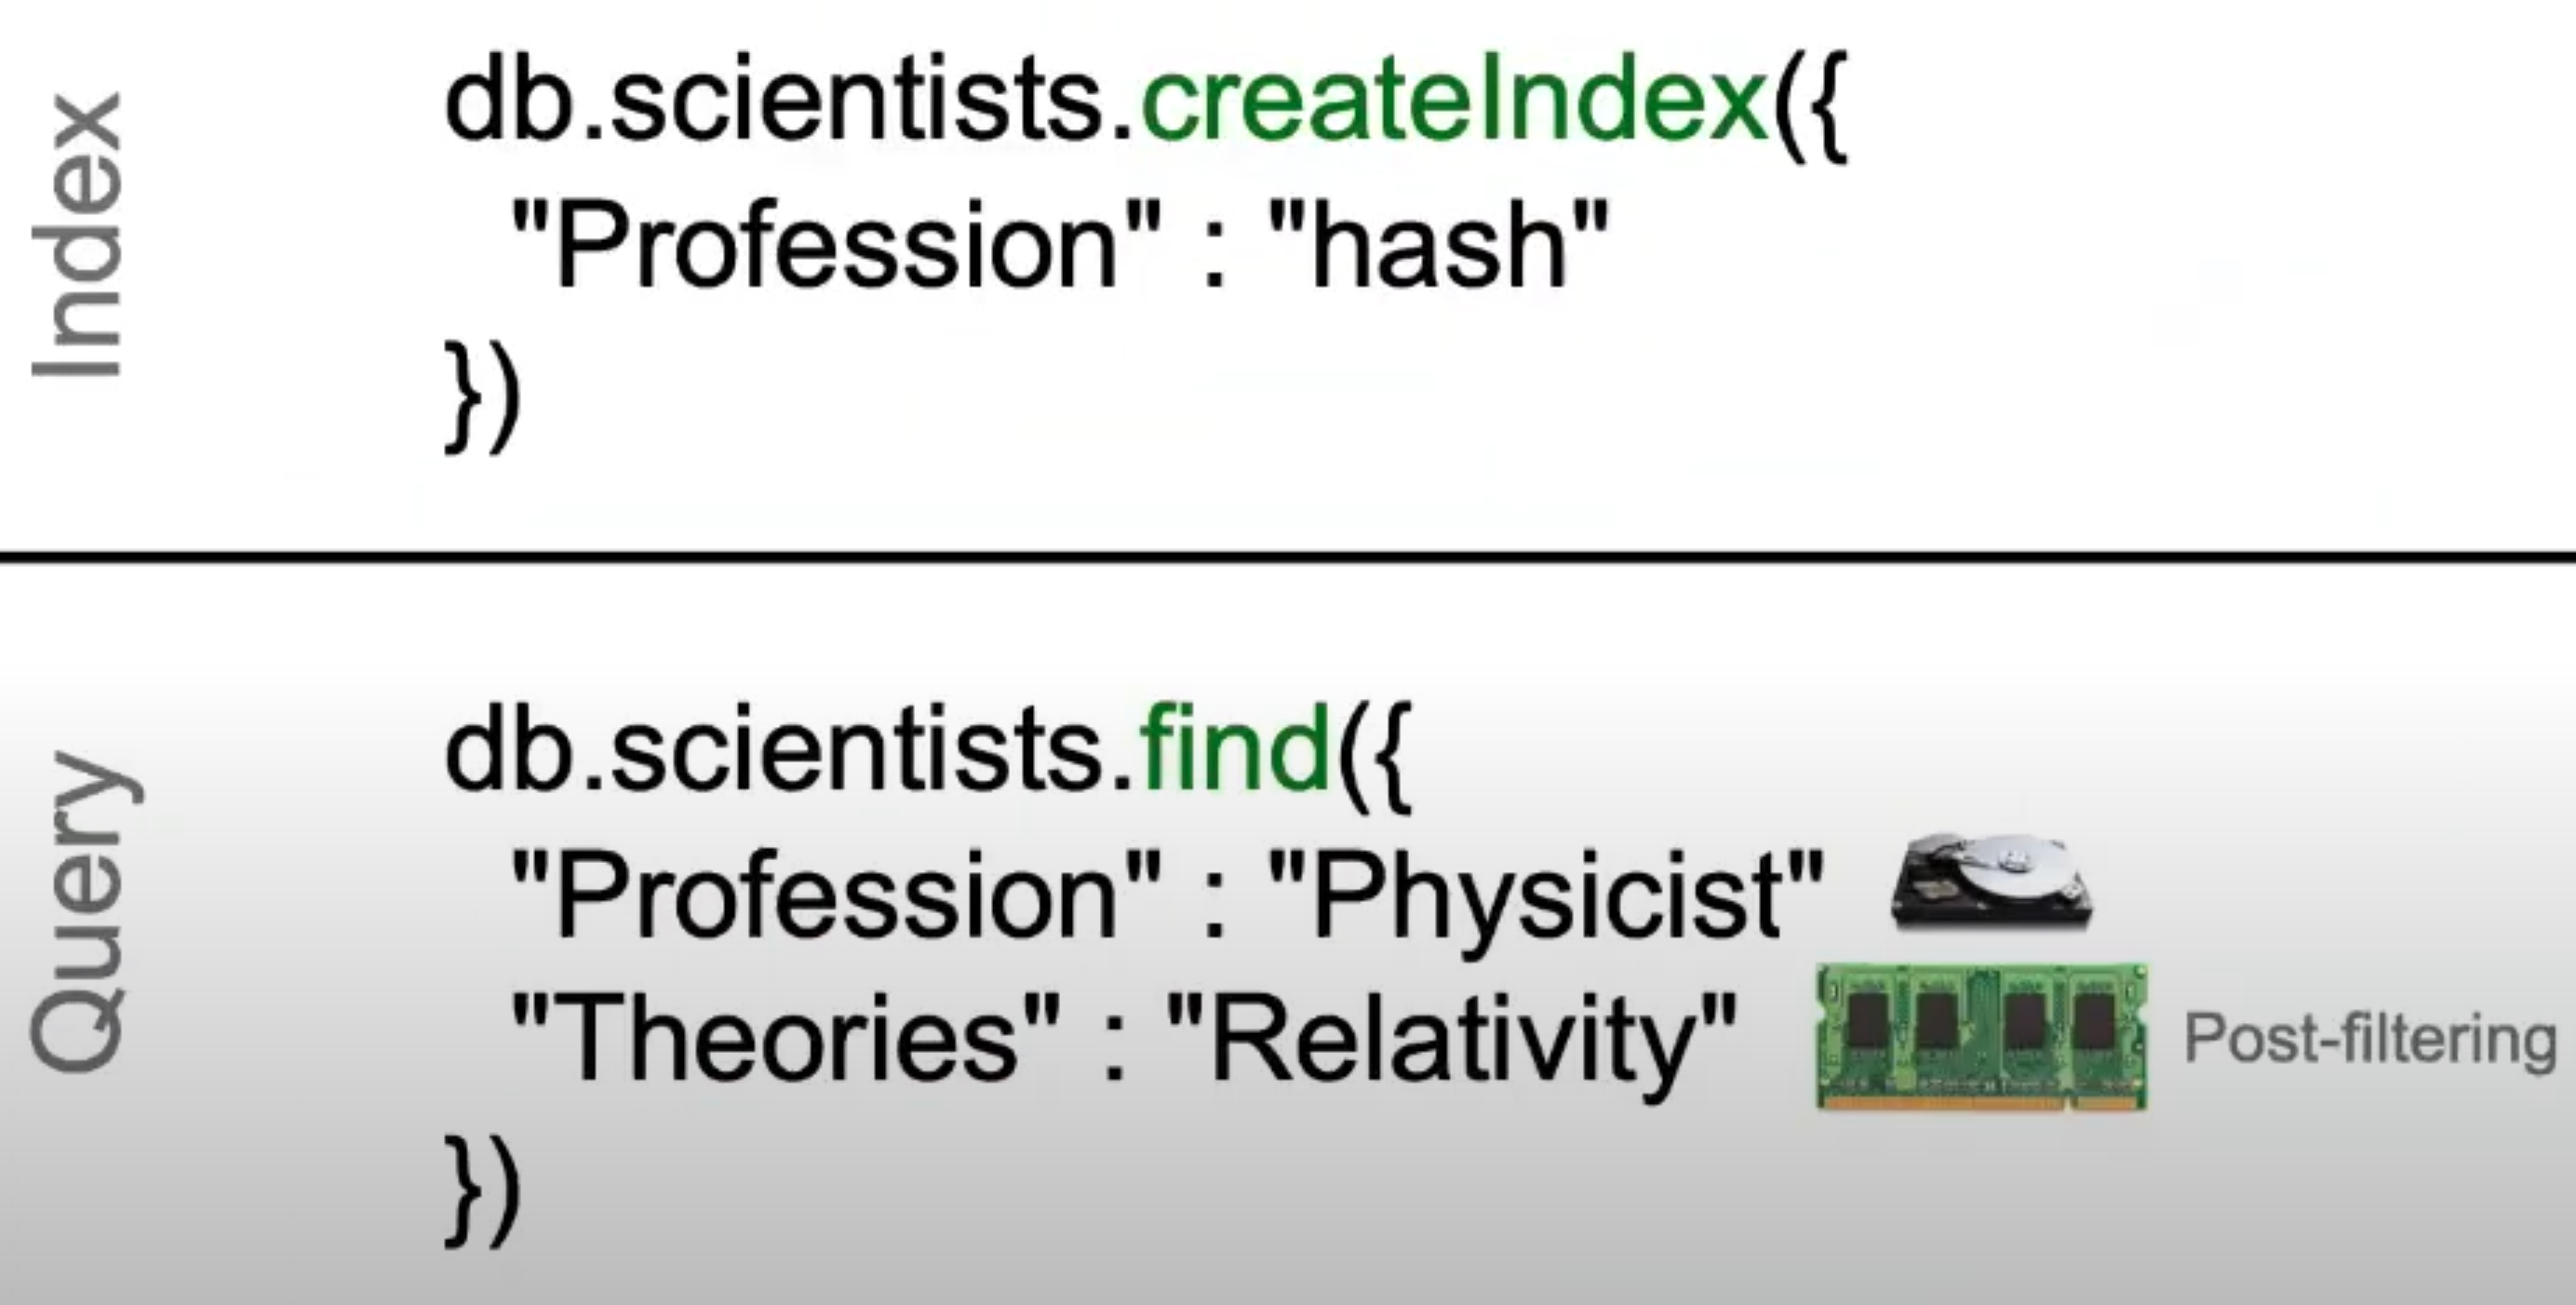
\includegraphics[width=0.5\textwidth]{Figures/IndexCreationandQuery.png}
    \caption{When creating a hash index function for one element of a document, here "Profession", then when querying the list of documents, the "Profession" is already filtered with the hash indexing, but any other filtering will be performed on the retrieved collection of documents.}
\end{figure}

You can also create and query compound indices as we have seen before:
\begin{lstlisting}[style=neutral]
db.scientists.createIndex({
    "Birth" : 1,
    "Death" : 1
})

db.scientists.find({
    "Birth" : 1887,
    "Death" : 1946
})
\end{lstlisting}

Now we can also implement range lookups:
\begin{lstlisting}[style=neutral]
db.scientists.createIndex({
    "Birth" : 1
})

db.scientists.find({
    "Birth" : {"$gte":1946}
})
\end{lstlisting}